\chapter{Introduction}

Computer systems have become an integral part of our daily life being used in various environments (such as homes, hospitals, factories) and application areas (such as medical devices, aircraft flight control, weapons, and nuclear systems). The increasing reliance of critical applications on information processing makes it vital to verify the soundness and safety of the computer systems because failure in these systems could be disastrous leading to financial loss, loss of life, or damage to the environment. To address this issue, formal verification comes into play. Formal verification is the process of mathematically proving or disproving the correctness of a system with respect to certain requirements or properties.

One of the most successful and powerful methods for formal verification is symbolic model checking. Symbolic model checking using induction-based techniques such as IC3/PDR~\cite{Een2011:PDR} and $k$-induction~\cite{SheeranSS00} can often determine whether safety properties hold of complex finite or infinite-state systems.  Model checking tools are attractive both because they are automated, requiring little or no interaction with the user, and if the answer to a correctness query is negative, they provide a counterexample to the satisfaction of the property.  These counterexamples can be used both to illustrate subtle errors in complex hardware and software designs~\cite{hilt2013,McMillan99:compositional, Miller10:CACM} and to support automated test case generation~\cite{Whalen13:OMCDC, You15:dse}.
In the event that a property is proved, however, it is not always clear what level of assurance should be invested in the result.  Given that these kinds of analyses are performed for safety- and security-critical software, this can lead to overconfidence in the behavior of the fielded system.  It is well known that issues such as vacuity~\cite{Kupferman03:Vacuity} can cause verification to succeed despite errors in a property specification or in the model. Even for non-vacuous specifications, it is possible to over-constrain the specification of the {\em environment} in the model such that the implementation will not work in the actual operating environment. 
%In such cases, a system or subsystem component will not exhibit the expected behavior in the operating environment although the analyst gains over-confidence or false assumption on the correctness of the system, which may bring about serious damage. Therefore, the level of feedback provided by the tool to the user matters.

At issue is the level of feedback provided by the tool to the user. In
most tools, when the answer to a correctness query is positive, no
further information is provided. What we would like to provide is
traceability information, an {\em inductive validity core} (IVC), that explains
the proof, in much the same way that a counterexample explains the
negative result. This is not a new idea: UNSAT cores~\cite{zhang2003extracting}
provide the same kind of information for individual SAT or
SMT queries, and this approach has been lifted to bounded analysis
for Alloy in~\cite{Torlak08:cores}. What we propose is a generic and efficient
mechanism for extracting supporting information, similar to an UNSAT
core, from the proofs of safety properties using inductive techniques
such as PDR and $k$-induction. Because many
properties are not themselves inductive, these proof techniques
introduce lemmas as part of the solving process in order to strengthen
the properties and make them inductive. Our technique allows
efficient, accurate, and precise extraction of inductive validity cores
even in the presence of such auxiliary lemmas. The idea lifts UNSAT cores~\cite{zhang2003extracting}
to the level of sequential model checking algorithms using induction.  Informally, if a model is viewed as a conjunction of constraints,
a minimal IVC (MIVC) is a set of constraints that is sufficient to construct a proof such that if any constraint is removed, the property is no longer valid.

\section{Objectives and Intended Contributions}

The IVC idea makes a lot of useful system analyses/engineering tasks possible and more efficient. Specifically, it is useful when the validity of a safety requirement has been stablished by the model checker. In this case, IVCs provide usable information both formal and human-understandable that explains why the requirement is satisfied. Such information is valuable in analyzing safety-critical systems and can be used for many purposes in the software verification process, including at least the following:
\begin{description}
    \item[Vacuity detection:] The idea of syntactic vacuity detection (checking whether all subformulae within a property are necessary for its satisfaction) has been well studied~\cite{Kupferman03:Vacuity}.   However, even if a property is not syntactically vacuous, it may not require substantial portions of the model.  This in turn may indicate that either a.) the model is incorrectly constructed or b.) the property is weaker than expected.  We have seen several examples of this mis-specification in our verification work, especially when variables computed by the model are used as part of antecedents to implications.
    \item[Completeness checking:] Closely related to vacuity detection is the idea of {\em completeness checking}, e.g., are all atoms in the model necessary for at least one of the properties proven about the model?  Several different notions of completeness checking have been proposed~\cite{chockler_coverage_2003, kupferman_theory_2008}, but these are very expensive to compute, and in some cases, provide an overly strict answer (e.g., checking can only be performed on non-vacuous models for~\cite{kupferman_theory_2008}).  
    \item[Traceability:] Certification standards for safety-critical systems (e.g.,~\cite{DO178C, MOD:00-55}) usually require {\em traceability matrices} that map high-level requirements to lower-level requirements and (eventually) leaf-level requirements to code or models.  Current traceability approaches involve either manual mappings between requirements and code/models~\cite{SimulinkTraceability} or a heuristic approach involving natural language processing~\cite{Keenan12:Tracelab}.  Both of these approaches tend to be inaccurate.  For functional properties that can be proven with inductive model checkers, inductive validity cores can provide accurate traceability matrices with no user effort.
    \item[Symbolic Simulation / Test Case Generation:]  Model checkers are now often used for symbolic simulation and structural-coverage-based test case generation~\cite{SimulinkDesignVerifier,Whalen13:OMCDC}.  For either of these purposes, the model checker is supposed to produce a witness trace for a given coverage obligation using a ``trap property'' which is expected to be falsifiable.  In systems of sufficient size, there is often ``dead code'' that cannot ever be reached.  In this case, a proof of non-reachability is produced, and the IVC provides the reason why this code is unreachable.
\end{description}
\noindent Nevertheless, to be useful for these tasks, the generation
process must be efficient and the generated IVC must be
accurate and precise (that is, sound and close to minimal).  The requirement for accuracy is obvious; otherwise the ``minimal'' set of model elements is no longer sufficient to produce a proof, so it no longer meets our IVC definition.  Minimality is important because (for traceability) we do not want unnecessary model elements in the trace matrix, and (for completeness) it may give us a false level of confidence that we have enough requirements.

%\ela{should we add this: (?)}
In addition, %\fixed{ a property can have as many unique minimal IVC sets as the possible paths through which it can be proved. Therefore,}
we are also interested in {\em diversity}:  how many different IVCs can be computed for a given property and model? Requirements engineers often talk about ``the traceability matrix'' or ``the satisfaction argument''.  If proofs are regularly diverse, then there are potentially many equally valid traceability matrices, and this may lead to changes in traceability research. 
It is often the case that there are multiple MIVCs for a given property.  In this case, computing a single IVC provides, at best, an incomplete picture of the traceability information associated with the proof.  Depending on the model and property to be analyzed, there is often substantial diversity between the IVCs used for proof, and there can also be a substantive difference in the size of a {\em minimal} IVC and a {\em minimum} IVC, which is the (not necessarily unique) smallest MIVC.
 If {\em all} MIVCs can be found, then several additional analyses can be performed:
\begin{description}
    \item [Coverage Analysis:] MIVCs can be used to define coverage metrics by examining the percentage of model elements required for a proof.  However, since MIVCs are not unique, there are multiple, equally legitimate coverage scores possible.  Having \emph{all} MIVCs allows one to define additional metrics: coverage of MAY elements, coverage of MUST elements, as well as policies for the existing MIVC metric: e.g., choose the smallest MIVC.
    \item [Optimizing Logic Synthesis:]  synthesis tools can benefit from MIVCs in the process of transforming an abstract behavior into a design implementation. A practical way of calculating all MIVCs allows to find a minimum set of design elements (optimal implementation) for a certain behavior. Such optimizations can be performed at different levels of synthesis.
    \item [Impact Analysis:] Given all MIVCs, it is possible to determine which requirements may be falsified by changes to the model.  This analysis allows for selective regression verification of tests and proofs: if there are alternate proof paths that do not require the modified portions of the model, then the requirement does not need to be re-verified.
    \item [Robustness Analysis:] It is possible to partition the model elements into MUST and MAY sets based on whether they are in every MIVC or only some MIVCs, respectively.  This may allow insight into the relative importance of different model elements for the property.  For example, if the MUST set is empty, then the requirement has been implemented in multiple ways, such as would be expected in a fault-tolerant system.
        %Moreover, examining the diversity of all MIVCs could lead to changes in how traceability~\cite{cleland2007best} is performed and managed in critical systems.
\end{description}

\noindent In addition, the Requirements Engineering community is keenly interested in approaches to manage requirements traceability.  In most cases, it is assumed that there is a single ``golden'' set of trace links that describes how requirements are implemented in software~\cite{COEST,hayes2003improving,cleland2007best}. However, if there are multiple MIVCs, then it is possible that there are several equally valid sets of trace links.  Examining the diversity of all MIVCs could lead to changes in how traceability is performed for critical systems.

\subsection{Contributions and Evaluation}
First, we propose a new method for extracting a single IVC from the inductive proof of a given property. This method is intended to be very efficient and impose a negligible overhead on the verification process.
Then, we propose a new method for computing \emph{all} MIVCs that is {\em always} minimal for decidable model checking problems and {\em usually} (and detectably) minimal for model-checking problems that are generally undecidable. We would like to evaluate the usability of our idea by examining its different applications.
The contributions of the work are therefore as follows:
\begin{itemize}
    \item We present a fast technique for extracting inductive validity
      cores from an inductive verification of a safety property over a sequential model involving lemmas.
    \item An algorithm for computing all minimal IVCs with a proof of correctness and completeness of the algorithm.
    \item We formalize all the techniques and present their implementations in the JKind model checker~\cite{jkind}.
    \item We present an experiment over our implementation and measure the efficiency, minimality, and robustness of the IVC generation process.
    %\item An evaluation of the algorithm for performance and diversity of result sets against a benchmark suite.
   \item A family of coverage metrics for formal verification based on \emph{minimal} Inductive Validity Cores (MIVCs).  Most of the proposed metrics are {\em proof preserving},
\item A discussion of the relationship between proof-based metrics and mutation-based metrics, including a proof of equivalence between non-deterministic mutation coverage and one of the proof-based metrics.
\item An experiment that compares our proof-based metrics against a state of the art mutation-based notion of completeness.
    \item We examine how the notion of IVCs changes the way traceability is perceived, established, maintained, and used.
\end{itemize}


%\section{State of the Art}
%Our work builds on top of a substantial foundation provided by special tools known as constraint solvers. Constraint solving is a powerful mathematical method that allows the computer to solve a problem formulated by the user. Many verification problems can be reduced to constraint satisfaction problems and solved with tools known as SMT  solvers.  A lot of useful formal methods are built on top of SMT solvers, such as model checking algorithms, abstraction techniques, and proof-certificate generation. There is significant amount of valuable research on these topics in the literature. Although such reasoning techniques are helpful, they are not expressive enough to provide good insights into the quality of a system or specification. With the IVC idea, we are able to bridge the gap between verification techniques and the user insight into the results provided by the tools. The goal behind this idea is different from existing applications of constraint solving. The IVC idea shares many similarities with existing approaches for computing proof certificates, and in fact the IVC algorithm performs this computation as well. However, there is a substantive difference; to find a guaranteed minimal set of certificates, it is usually necessary to find new proofs involving new invariants not used in the original proof, which existing techniques do not deal with.
 

 
%% We put the image here so it shows up side-by-side with fig:ex-after
%\begin{figure}[t]
%\centering
%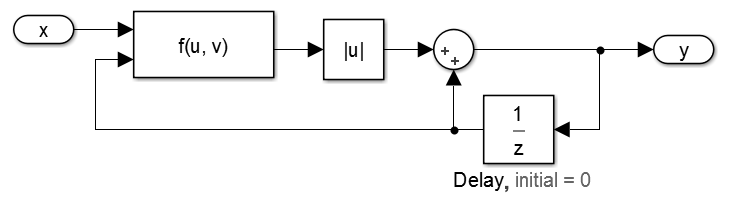
\includegraphics[width=\columnwidth]{figs/simulink.png}
%{\smaller
%\begin{verbatim}
%node filter(x : real) returns (a, b, y : real);
%let
%  a = f(x, 0.0 -> pre y);
%  b = if a >= 0.0 then a else -a;
%  y = b + (0.0 -> pre y);
%tel;
%\end{verbatim}
%}
%\vspace{-0.1in}
%\caption{Model with property $y \geq 0$, before IVC analysis}
%\label{fig:ex-before}
%\end{figure}